\documentclass[sigconf]{acmart}

\usepackage[]{graphicx}
\usepackage[]{color}
\makeatletter
\def\maxwidth{ %
 \ifdim\Gin@nat@width>\linewidth
 \linewidth
 \else
 \Gin@nat@width
 \fi
}
\makeatother


\usepackage{subfig}
\usepackage{listings}
\makeatletter
\newenvironment{kframe}{%
 \def\at@end@of@kframe{}%
 \ifinner\ifhmode%
 \def\at@end@of@kframe{\end{minipage}}%
 \begin{minipage}{\columnwidth}%
 \fi\fi%
 \def\FrameCommand##1{\hskip\@totalleftmargin \hskip-\fboxsep
 \colorbox{shadecolor}{##1}\hskip-\fboxsep
 % There is no \\@totalrightmargin, so:
 \hskip-\linewidth \hskip-\@totalleftmargin \hskip\columnwidth}%
 \MakeFramed {\advance\hsize-\width
 \@totalleftmargin\z@ \linewidth\hsize
 \@setminipage}}%
 {\par\unskip\endMakeFramed%
 \at@end@of@kframe}
\makeatother

\usepackage{alltt}
\usepackage{multicol}
\pagestyle{plain}
%\usepackage{amsmath}
%\usepackage{caption} 
%\captionsetup[table]{skip=3pt}

\AtBeginDocument{%
 \providecommand\BibTeX{{%
 \normalfont B\kern-0.5em{\scshape i\kern-0.25em b}\kern-0.8em\TeX}}}

\setcopyright{acmcopyright}
\copyrightyear{2019}
\acmYear{2019}
\acmDOI{10.1145/1122445.1122456}

\acmConference[DYNAMICS '19]{DYNAMICS '19: DYnamic and Novel Advances in Machine Learning and Intelligent Cyber Security Workshop}{December 09--10, 2019}{San Juan, PR}
\acmBooktitle{DYNAMICS '19: DYnamic and Novel Advances in Machine Learning and Intelligent Cyber Security Workshop,
 December 09--10, 2019, San Juan, PR}
\acmPrice{15.00}
\acmISBN{978-1-4503-9999-9/18/06}
\IfFileExists{upquote.sty}{\usepackage{upquote}}{}

\begin{document}

\title{Traffic Generation using Containerization for Machine Learning}

\author{Henry Clausen}
%\authornote{Both authors contributed equally to this research.}
\email{henry.clausen@ed.ac.uk}
\affiliation{%
  \institution{University of Edinburgh}
    \city{Edinburgh, UK}
}

\author{Robert Flood}
\email{s1784464@ed.ac.uk}
\affiliation{%
  \institution{University of Edinburgh}
      \city{Edinburgh, UK}
}

\author{David Aspinall}
\affiliation{%
  \institution{University of Edinburgh}
      \city{Edinburgh, UK}
  \\ \institution{The Alan Turing Institute}
      \city{London, UK}
}



\begin{abstract}

\end{abstract}

\keywords{Network security, datasets, machine learning, intrusion detection}

\maketitle

\section{Introduction}


\dots \dots

\dots \dots

\dots \dots

This work provides the following contributions:

\begin{enumerate}
 \item We present a novel network traffic generation framework that is designed to improve several shortcomings of current datasets for NIDS evaluation. This framework is openly accessible for researchers and allows for straightforward customization.
 \item We define four new requirements a network intrusion dataset should fulfil in order to be suitable to train machine-learning based intrusion detection methods. 
 %\item how to build new modules that can be added to the existing framework, and how this procedure enables data generation that is more suitable for data-driven methods than currently available datasets.
 \item We perform a number of experiments to demonstrate the suitability and utility of our framework. 
\end{enumerate}

\subsection{Outline}

The remainder of the paper is organized as follows. Section \ref{Sec:background} discusses existing NIDS datasets and the problems that arise during their usage as well as background information about network traffic data formats and virtualization methods. The section concludes with a set of requirements we propose to improve the training and evaluation of machine-learning-based methods. Section \ref{Sec:Design} describes the general design of our framework, and how it improves on the discussed problems in existing datasets. We also discuss a specific example in detail. Section \ref{Sec:Experiments} discusses several experiments to validate the improvements and utility our framework provides. 
Section \ref{Sec:Conclusion} concludes the results and discusses limitations of our work and directions for future work.


\section{Background}\label{Sec:background}

\subsection{Data formats}

\subsection{Related work and existing datasets}




\subsection{Problems in modern datasets}\label{Sec:problems}



\subsection{Containerization with Docker}
%\textcolor{red}{to do:need to improve

\subsection{MiniNet}





\section{Dataset Requirements}\label{Sec:require}


\paragraph{Variation}
 
\paragraph{Ground truth} 

\paragraph{Modularity}

\paragraph{Scalability} 


\section{Design}\label{Sec:Design}

\subsection{Modes of Operation}


\begin{figure}
 \centering 
 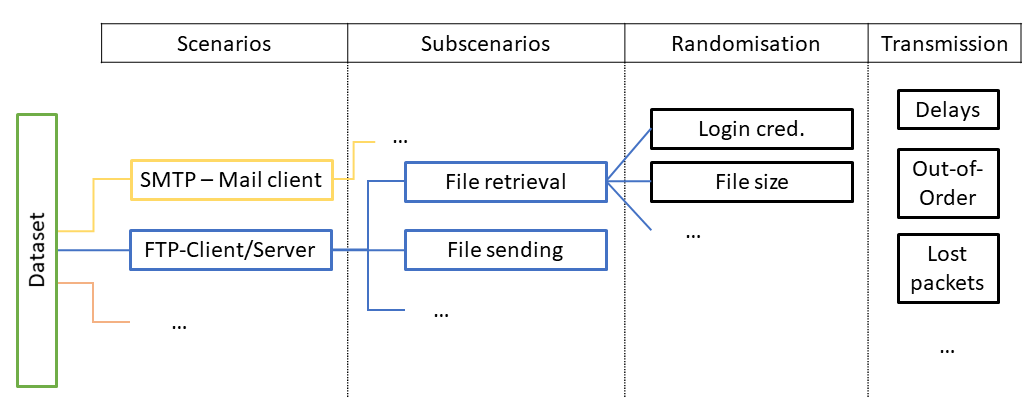
\includegraphics[width=0.480\textwidth]{images/scenario_branching.PNG}
 \caption{Visualization of the different levels at which traffic variation is introduced in DetGen.}
 \label{Fig:branching}
\end{figure}


\subsection{Scenarios and subscenarios}
\label{Sec:Scenarios}

\subsection{Randomization}\label{Sec:randomsubscen}

\subsection{Network transmission}\label{Sec:Netrand}


\subsection{Implementation Process}

 
\subsection{Implemented scenarios}\label{Sec:ExistScen}


\begin{figure}%[h!]
\centering
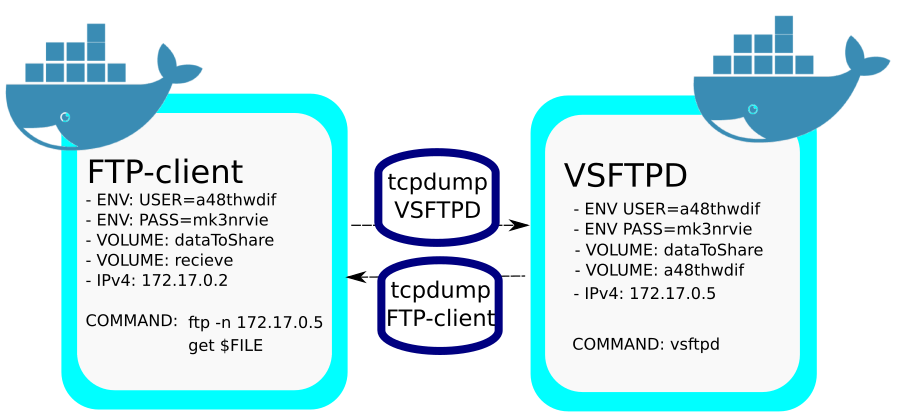
\includegraphics[width=0.49\textwidth]{images/ftp_new1.png}
\caption{Diagram of FTP scenario}
\end{figure}


\subsection{Network-simulation mode}

\subsubsection{Dataset coalescence}\label{Sec:datasetcreation}


\subsection{Network-simulation mode}




\section{Validation experiments}\label{Sec:Experiments}

A framework that generates network traffic does not necessarily provide realistic and useful data. To evaluate the utility of our Docker framework, we construct a series of experiments. We have two goals in mind. First, we want to demonstrate that the traffic generated is sufficiently representative of real-world traffic.
Second, we want to demonstrate that having a framework to continually generate data compared to static datasets benefits evaluating the efficacy of intrusion detection systems.

The first experiment provides a general verification of the reproducability of our framework, which is required for guarantee the ground truth of the produced data. The second experiment demonstrates that the WAN-characteristics we emulate for our data make it quasi non-distinguishable from real WAN traffic. Our third experiment then demonstrates the advantage of unlimited data generation capabilities for training ML-based traffic classification.


\subsection{Reproducible scenarios}\label{Sec:deterministic}

To provide ground truth, we have to guarantee that our implemented scenarios and subscenarios are consistent and reproducible upon repeated execution. This applies both to consistency for external influences on the host, such as increased computational load, as well as internal consistency of the implemented script execution. 

It is impossible to guarantee that each scenario will produce a truly `deterministic', or repeatable, output due to differences in network conditions, computational times, or input. Instead, we aim for our data to be \textit{reproducible up to networking and computational differences}. This means that when running a scenario multiple times, we expect the quantities of most packets to be largely identical. We do expect some packets to exhibit greater variation due to non-determinism in the underlying protocols, Fig. \ref{fig:size1} outlines this behavior in terms of interarrival times and packet sizes. 

\begin{figure}
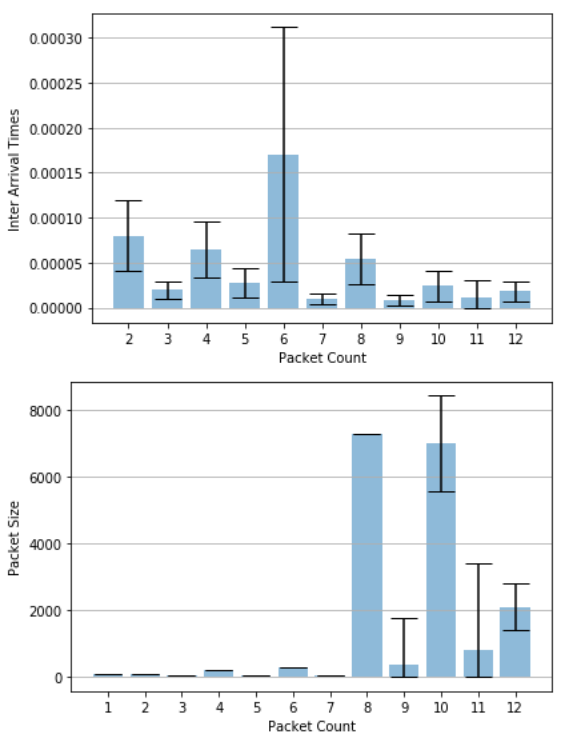
\includegraphics[width=0.45\textwidth]{images/combined3.png} % first figure itself
\caption{Means of IATs \& packet sizes along with standard deviation bars for the first twelve packets in the Apache scenario.}
\label{fig:size1}
\end{figure}

To measure how consistent our scenarios are, we generate 500 \texttt{.pcap} files for three different implemented scenarios, namely the Apache, the VSFTPD, and the SSH scenario. These were generated consecutively under different host CPU load. We did not apply any delays or other NetEm traffic controls.

We assess the consistency of a scenario across different \texttt{.pcap} files by comparing all generated \texttt{.pcap} files pairwize. We measure this by the similarity of the connections captured. 

To test the similarity of two connections, we extract the sample distributions of the packet interarrival times and packet sizes overall, upstream and downstream. We define two connections as similar if the two distributions for each of these quantities pass an equality test. We use the two-sample Kolmogorov-Smirnov (K-S) test, a non-parametric statistical test for the equality of two continuous one-dimensional distributions \cite{massey1951kolmogorov}, with a p-value of $0.01$. 

As all tested files passed this similarity test, we conclude that these scenarios yield consistent and reproducible results. As other scenarios follow the same setup and launch commands, we expect the results to stay the same as long as the involved containers are consistent in their behavior.




% Need to edit these sections to provide a single context for both the artificial delays & classification

\subsection{Explorating Artificial Delays}


%In order for results drawn from datasets generated using our Docker framework to generalize, it is necessary to ensure that the qualities of our generated traffic are sufficiently similar to those of real-world traffic. However, it is not immediately clear if the traffic generated by our suite of Docker containers satisfies this condition. 

%Probably need to further justify why we chose to experiment using IATs specifically rather than, say, packet corruption

Most traffic our framework generates is transported over Docker's virtual network and therefore does not succumb to problems associated with normal network congestion, such as packet loss, corruption and packets arriving out of order. A realistic dataset should include these phenomena, which is why we developed wrapping scripts that allow us to artificially add delays as well as packet loss and corruption, using NetEm. Choosing the parameters is not straightforward; it is not clear how close to real-world traffic such network emulation techniques are. This is especially true for packet delays, which are described by continuous distributions and often have temporal correlation.

Furthermore, the high effective bandwidth of the Docker virtual network resulted in traffic with extremely short inter-arrival times (IATs, defined as the time between two packet arrivals). Therefore, we devote considerable time to demonstrating that it is possible for traffic generated by our Docker framework to conform to real-world IAT distributions when altered using NetEm.

% Use subsubsections for results/datasets?

\subsubsection*{Datasets} We create two classes of datasets, one which is representative of `real-world' traffic, and one which has been generated from our Docker framework. For simplicity, we only consider datasets consisting of FTP traffic.

For the real-world dataset, we set up a containerized VSFTPD server running on a \emph{Google Compute} virtual machine located in the Eastern United States, and a containerized FTP client on our local host. We then ran a series of our scripted interactions between the two machines, generating 834 megabytes of data in 250964 packets. These interactions consisted of several FTP commands with various network footprints. We collect all data transmitted on both the server and the client. We call this data the \textit{Non-Local} dataset.

We then repeat this process using the same container setup, but across the Docker virtual network on a local machine. We repeat this process several times, generating several \textit{Local} datasets under a variety of emulated network conditions, discussed in Section \ref{Sec:method1}. Our \textit{Local} datasets vary slightly in size, but are all roughly 800 megabytes with 245000 packets. %We illustrate this setup in Fig. \ref{Fig:google}.

%\begin{figure*}
%\centering
%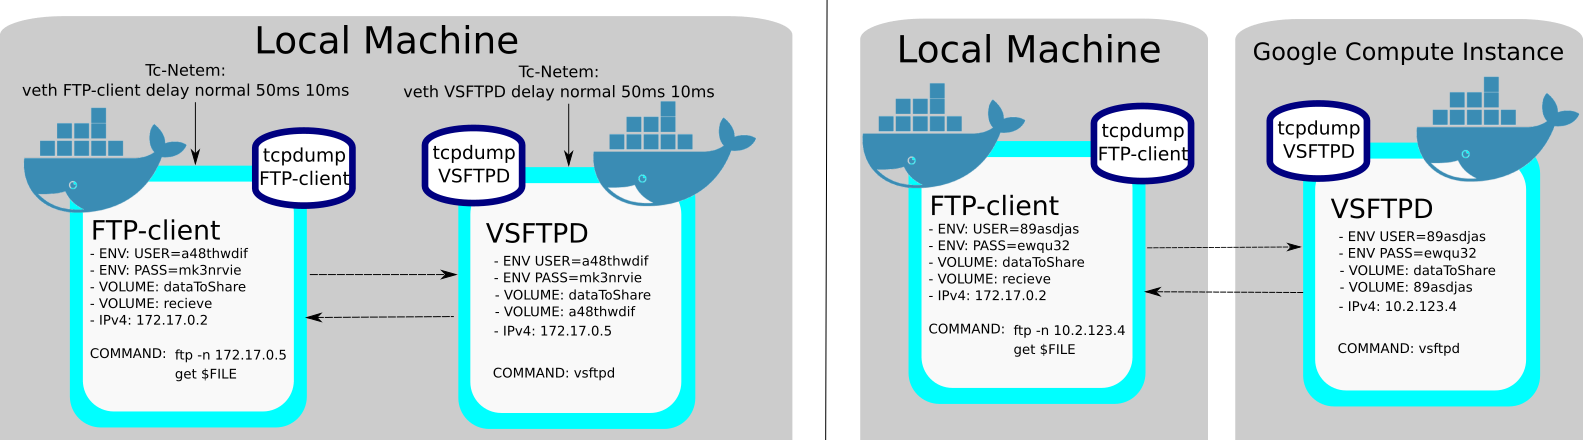
\includegraphics[width=0.8\textwidth]{images/ftp_new2.png}
%\caption{Diagram of our Dataset Generation Architecture}
%\label{Fig:google}
%\end{figure*}

\subsubsection*{Methodology}
\label{Sec:method1}


NetEm allows us to introduce packet delays according to a variety of distributions, namely uniform, normal, Pareto and Paretonormal\footnote{This Paretonormal distribution is defined by the random variable $Z = 0.25*X + 0.75*Y$, where $X$ is a random variable drawn from a normal distribution and $Y$ is a random variable drawn from a Pareto distribution.}. Furthermore, NetEm adds delays according to modifiable distribution tables, and so it is trivial for us to add a Weibull distribution, which along with Pareto distributions have been shown to closely model packet IATs \cite{arfeen2013role,paxson1995wide}.
In total, we test the efficacy of four distributions to model inter-arrival times --- normal, Pareto, Paretonormal and Weibull. 
 
We generate several \textit{Local} datasets by delaying traffic according these distributions, performing an exhaustive grid search over their means and standard deviations. Initial experiments revealed that introducing delays with a mean in the range of 40 ms to 70 ms produced the best results. Setting the jitter of the distribution too high resulted in the repeated arrival of packets out of order, therefore we further limit the grid search to jitter values in 5ms intervals up to half of the value of the mean. In total, we generate 88 \textit{Local} datasets.

Our goal is to discover the \textit{Local} dataset whose packet timings most closely resemble those of our \textit{Non-Local} dataset. To do this, we extract the IATs and packet sizes from our datasets on a packet-by-packet basis and store these results in arrays. We measure the similarity between two of these arrays by training a Random Forest classifier to distinguish between them. We say that if the Random Forest correctly classifies each packet with a success rate of only 50\% then it is no better than randomly guessing and, as such, the inter-arrival times of these two arrays are indistinguishable from one another for the Random Forest.

To perform this measurement, we concatenate one \textit{Local} dataset array with our \textit{Non-Local} dataset array, label the entries and then shuffle the rows. We proportion this data into a training set and a testing set using an 80-20 split. We then feed this training data into a Random Forest with 1000 trees and fixed seed, and then record the accuracy of this Random Forest on the test set. We repeat this process for every single \textit{Local} dataset.

\subsubsection*{Results}


\begin{figure}
\captionsetup{justification=centering}
\centering
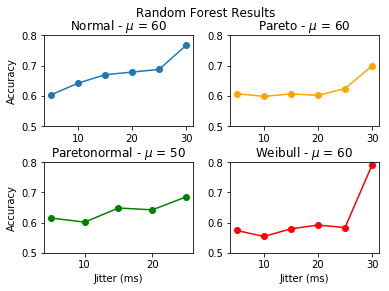
\includegraphics[width=0.45\textwidth]{images/1-plot_exp1.png}
\caption{Results of Random Forest Classifier for a given distribution at the best performing delay mean $\mu$. Note that a score of .5 indicates total indistinguishability.}
\label{Fig:rf_graph}
\end{figure}

Table \ref{tab:results-iat_rf} summarizes the values of the mean and jitter for a given distribution that produced the worst results from the random forest classifier.


\begin{table}[ht!]
\begin{center}
\begin{small}
\begin{sc}
\begin{tabular}{ccccc}
\hline
Distribution & Mean & Jitter & RF Accuracy\\
\hline
No Delays (Baseline) & 0 & 0ms & 0.8176 \\
Constant Delay & 40ms & 0ms & 0.6730 \\
Normal & 60ms & 5ms & 0.6028 \\
Pareto & 60ms & 10ms & 0.5979 \\
Paretonormal & 50ms & 10ms & 0.6015 \\
Weibull & 60ms & 10ms & 0.5540 \\
\hline
\end{tabular}
\end{sc}
\end{small}
\caption{Worst Random Forest accuracy rates for a given distribution}
\label{tab:results-iat_rf}
\end{center}
\vskip -4mm
\end{table}

To establish a baseline, we compare the traffic generated from our Docker scenario to that of the \textit{Google Compute} data with no added delays. In this case, the Random Forest was able to distinguish between the two datasets, achieving an accuracy of over 90\%. The classification accuracy is worsened considerably by introducing network delays, with the best results being achieved using a Weibull distribution with a mean of 60 ms and a jitter of 10 ms, leading to an accuracy of just $55\%$. Results for Pareto and Weibull distributions seem to yield consistent results for differing jitter values.
Although not completely indistinguishable, this proves that using NetEm we can emulate WAN properties very closely.

\subsection{Advantages of Dynamic Dataset Generation}
%The name needs to be changed, be clear what this verifies about our framework
% I suppose that this experiment verifies that being able to continually generate traffic with a variety of network traffic conditions is an important quality for a traffic generation framework. Moreover, the cited papers both used k-means classifiers as they did not have access to labeled datasets, whilst we were able to use a random forest because our dataset was labeled. So, the title could be something like 'Advantages of dynamic dataset generation with accurate ground truth in traffic classification'? A bit long winded.

Having examined whether our Docker framework is capable of emulating real-world IATs, we explore their utility in traffic classification to demonstrate the advantages that our framework provides compared to static, unlabeled datasets.

Machine-learning techniques are a popular tool for traffic classification, with many successful published classifiers. Furthermore, inter-packet arrival times have been shown to be a discriminative feature \cite{zander2005automated,nguyen2008survey}. However, these methods considered datasets consisting of completed traffic flows, limiting their use in, say, a stateful packet inspector. On-the-fly classifiers are also successful. Jaber et al. \cite{jaber2011can} showed that a K-means classifier can classify flows in real-time solely based on IATs with precision exceeding 90\% for most protocols within 18 packets. Similarly, Bernaille et al. \cite{bernaille2006traffic} demonstrated that a K-means classifier can precisely classify traffic within five packets using only packet size as a feature. 

 However, Jaber et al. \cite{jaber2011can} only evaluated their traffic classifier with training and testing data drawn from the same dataset containing traces of a single network; there is no measure of how this model may generalize to other networks with differing conditions. Furthermore, they were limited to using unsupervised machine learning algorithms to classify their traffic as their datasets had no ground truth. 

We attempt to replicate these results within our Docker framework with some adjustments. As we can generate a fully accurate ground truth, we attempt to segregate application flows based on their packet IATs using supervised learning techniques. Moreover, we then measure this model's ability to generalize by expanding our dataset to include traffic from networks with differing bandwidth and latency.

\subsubsection*{Data \& Preprocessing}

Our goal is to measure a classifier's ability to generalize across datasets. Therefore we construct two datasets using our Docker framework, both containing the same number of network traces from the same containers. 

For our first dataset, we generate \texttt{.pcap}-files, each containing traffic from one of 16 different classes: HTTP (Client \& Server), HTTPS (Client \& Server), RTMP (Client, Server \& Viewer), SSH (Client \& Server), FTP (Client \& Server), IRC (Client \& Server), SMTP, SQLi and DoS traffic. To prevent class imbalance, we generate 200 \texttt{.pcap}-files for each of the 16 classes, resulting in 3200 total files. To more accurately emulate potential network conditions, we use our NetEm scripts to apply a unique delay to every container involved in a scenario. These delays follow a Pareto distribution with random mean between 0 and 100 milliseconds and random jitter between 0 and 10 milliseconds. We then preprocess this data by removing all but the first 12 packets of each \texttt{.pcap}-file. We extract the 11 inter-arrival times separating the 12 packets, which act as our feature vectors. We collect these feature vectors for each class along with a class label, and store collected feature vectors from all 3200 \texttt{.pcap}-files in a 12 x 3200 array. We call this our \textit{Primary} dataset.

We then repeat this process to generate a second dataset, changing the properties of our emulated network. Again, we delay all traffic using a Pareto distribution, however, this time we select a random mean in the range of 100 to 500 milliseconds and random jitter between 0 and 50 milliseconds. The subsequent preprocessing of our data remains unchanged. We call this our \textit{Secondary} dataset.

\subsubsection*{Methodology}

\label{Sec:exp2_method}
First, we attempt to reproduce the results presented by Jaber et al. \cite{jaber2011can} by training a Random Forest with 100 trees to classify application flows based on packet IATs. We do this by proportioning our Primary dataset into training and testing sets using an 80-20 split. We then train and test our Random Forest repeatedly, first considering the classification accuracy based on the IATs of only the first two packets, then the first three packets and so on, up to 12 packets. We record the resulting confusion matrix for each round and calculate the precision and recall rates of our classifier.

Having trained the classifier, we measure its ability to generalize by repeating the above experiment, but replacing the test set with the Secondary dataset.


\subsubsection*{Results}

%\begin{figure*}
%\begin{multicols}{2}
%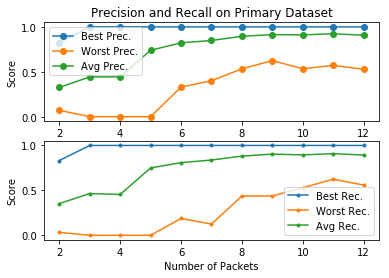
\includegraphics[width=linewidth]{images/primary_prec.png} % first figure itself
%\caption{\centering{Precision \& Recall %for Primary Dataset}}
%\end{multicols}
%\begin{multicols}{2}
%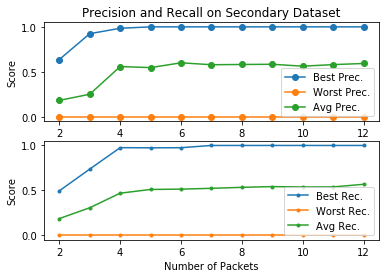
\includegraphics[width=linewidth]{AC%SAC_DYNAMICS/images/secondary_prec.png} % second figure itself
%\caption{\centering{Precision \& Recall %for Secondary Dataset}}
%\end{multicols}
%\end{figure*}

 After each run of our Random Forest on our Primary dataset, we gather the True Positive ($T_{P}$), False Positive ($F_{P}$) and False Negative ($F_{N})$ rate for each class. We then calculate their precision, defined as $ \frac{T_P}{T_P + F_P}$, and recall, defined as $ \frac{T_P}{T_P + F_N}$, values. in Fig. \ref{Fig:Primary}, we see that our average precision and recall across the classes exceeds 0.9 after 10 IATs. Furthermore, after 12 packets our DoS and SQLi data is classified with precision and recall rates of 1.0 and 1.0 and 0.9462 and 0.9322 respectively.

These results does not hold when we test the classifyer on our Secondary dataset. As seen in Fig. \ref{Fig:Primary}, we see a substantial decrease in our average precision and recall rates, achieving a maximum of 0.5923 and 0.5676 respectively. Moreover, after four packets, increasing the number of IATs in our dataset provides little additional benefit. Although some services generalized well, such as IRC-client and IRC-server, others failed to be classified, with every single SMTP feature being classified as HTTP-client. We also see a substantial drop-off in the classification of malicious traffic, with the precision rates of DoS and SQLi data not exceeding 0.6.

These diverging results demonstrate the necessity of dynamic dataset generation for evaluation purposes. Researchers evaluating their methods only on a dataset with fixed properties such as the Primary dataset might receive overoptimistic results. The capability of generating two or more datasets with the same traffic classes, but otherwise differing properties, provides a more realistic evaluation.


\begin{figure}%[ht!]

\subfloat{%
 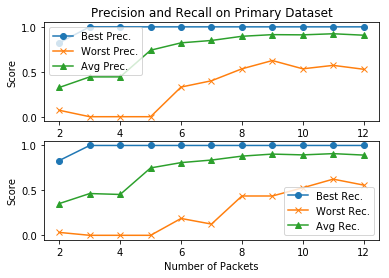
\includegraphics[width=0.4\textwidth]{images/bw_100_exp_3.png}
}

\subfloat{
 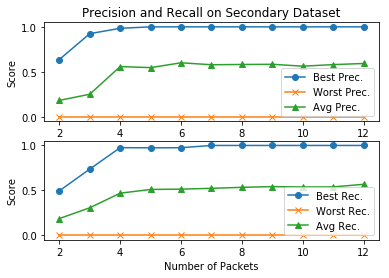
\includegraphics[width=0.4\textwidth]{images/bw_500_exp_3.png}
}

\caption{Results of Random Forest Classification on Primary dataset (Above) and Secondary dataset (Below)}
\label{Fig:Primary}
\end{figure}


\section{Conclusions}\label{Sec:Conclusion}

In this paper, we outlined four requirements a modern dataset has to fulfil to strengthen the training of intrusion detection systems. We then proposed a Docker framework capable of generating network intrusion datasets that satisfy these conditions. The major design advantage of this framework are the isolation of traffic scenarios into separate container arrangements, which allows the extension of new scenarios and detailed implementation of subscenarios as well as the capture of ground truth of the computational origins of individual traffic events. Furthermore, containerization enables the generation of traffic data at scale due to containers being light-weight and easily clonable.

We verified the realism of the generated traffic and the corresponding ground truth information with two experiments, and demonstrated the usefulness of the framework in another experiment.
Presently, our framework consists of 29 scenarios capable of producing benign and malicious network traffic. Several of these scenarios, such as the \emph{BitTorrent} or the \emph{Stepping-Stone} scenario, provide novel traffic data of protocols or behaviours that has not been widely available to researchers previously.


\subsection{Difficulties and limitations}

Our framework is building network traffic datasets from a small-scale level up by coalescing traffic from different fine-grained scenarios together. While this provides great insight into small-scale traffic structures, our framework will not replicate realistic network-wide temporal structures, such as port usage distributions or long-term temporal activity. These quantities would have to be statistically estimated from other real-world traffic beforehand to allow our framework to emulate such behavior reliably. Other datasets such as UGR-16 use this approach to fuse real-world and synthetic traffic and are currently better suited to build models of large-scale traffic structures.

Working with Docker containers can sometimes complicate the implementation of individual scenarios compared to working with VMs. Although several applications are officially maintained Docker containers that are free from major errors, many do not. For instance, in the \textit{BitTorrent} scenario, most common command line tools, such as \texttt{mktorrent}, \texttt{ctorrent} and \texttt{buildtorrent}, failed to actually produce functioning torrent files from within a container due to Docker's union filesystem. Furthermore, due to the unique way in which we are using these software packages, unusual configuration settings are sometimes needed. %As such, many 

Lastly, capturing \texttt{.pcap}-files from each container can quickly exceed available disc space when generating traffic at scale. Depending on specific research requirements, it is advizable to add filtering or feature extraction commands to the scenario execution scripts to enable traffic preprocessing in real-time.


\subsection{Future work}

Our traffic generation framework is designed to be expandable and there are many avenues for future work. The continual development of scenarios and subscenarios would improve the potential realism of datasets generated using the framework. The addition of more malicious scenarios would enable a more detailed model evaluation and improve detection rate estimation. 
Another future improvement for framework is to add scripts that emulate the usage activity of individual scenarios by a user or a network. 


Although ground truth for particular traffic traces is provided by capturing \texttt{.pcap}-files for each container individually, we have not implemented a labelling mechanism yet for the dataset coalescence process. Though not technically difficult, some thought will have to be put how such labels would look like to satisfy different research demands.
Furthermore, the Docker platform provides the functionality to collect system logs via the \texttt{syslog logging driver}. We plan on implementing their collection in the future, where they could act either as traffic labels providing more ground truth details, or act as a separate data source that complements the collected traffic.

We wish to publish this framework to a wider audience, allowing for further modification. This will be done using a GitHub repository, which contains both the implemented capture scenarios as well as the corresponding container images.


%Syslog logging driver
%add server to capture syslogs 

%https://docs.docker.com/config/containers/logging/syslog/

\section{Acknowledgments}

% https://epsrc.ukri.org/skills/students/dta/caseconvert/
We are grateful to  British Telecommunications PLC who are supporting the PhD research of the first
author in the UK EPSRC CASE scheme, giving invaluable guidance on the
needs and possibilities of intelligent security tools and their
evaluation.  Part of this paper draws on the 2019 MSc dissertation of
the second author.  %% FIXME: is it referenced?
Nikola Pavlov helped with some of the earlier implementation.  The
third author was supported by The Alan Turing Institute under the
EPSRC grant EP/N510129/1 and the Office of Naval Research ONR NICOP
award N62909-17-1-2065.

%We are grateful for our ongoing collaboration with our industry partners  on this topic area, who provided both ongoing support and guidance to this work. Discussions with them have helped reinforce the need for a better evaluation and understanding of the possibilities that new intelligent tools can provide.

%Full funding sources after currently blinded.

\bibliographystyle{ACM-Reference-Format}
 
\bibliography{DetGen_ext}

%\appendix

%\section{Protocol Coverage}

%We initially investigated the protocols and applications present in existing network traffic datasets. Our analysis includes CIC-IDS 2017 \cite{sharafaldin2018toward}, UNSW-NB15 \cite{moustafa2015unsw}, ICSX Botnet \cite{beigi2014towards} and Mawi \cite{fontugne2010mawilab}. We chose these datasets as they provide \texttt{.pcap}-files of their network traffic which enables us to more easily see what protocols are present. To do this, we used the Bro IDS tool to generate log files, listing the results in table \ref{tab:results-bro}.

%The protocols listed in table \ref{tab:results-bro} make up over 90\% of the benign traffic in these datasets. Moreover, although the ratio of protocols in datasets can differ significantly, we see some patterns: namely, protocols associated with general browser usage, such as HTTP, SSL, DNS, are the most common in each dataset. 

%\begin{table}[ht!]
%\begin{center}
%\begin{small}
%\begin{sc}
%\begin{tabular}{ccccc}
%\hline
%Protocol & UNSW-NB15 & ISCX & CIC-IDS 2017 & Mawi\\
%\hline
%HTTP & 196195 & 2372 & 276405 & 156179 \\
%SSL & 540 & 141 & 285760 & 591551 \\
%DNS & 372748 & 200009 & 1820105 & 1581858 \\
%X509 & 459 & 331 & 2758590 & Unknown \\
%FTP & 111685 & 1989 & 5540 & 278 \\
%SSH & 31320 & 434 & 5600 & 5503 \\
%IRC & 202 & 27 & 0 & Unknown \\
%SMTP & 44455 & 125 & 0 & 4601 \\
%\hline
%\end{tabular}
%\end{sc}
%\end{small}
%\vskip -2mm
%\caption{Bro Log Flow Count}
%\label{tab:results-bro}
%\end{center}
%%\vskip -4mm
%\end{table}



%We could base the ratios of protocols in our own dataset off of those found in an existing dataset where the traffic has been artificially generated. However, this would be problematic. In the case of CIC-IDS 2017, some protocols that make up a substantial amount of real-world traffic are glaringly omitted, such as BitTorrent or video streaming protocols. In contrast, although UNSW-NB15 contains a better range of protocols, only a small percentage of their web traffic is transmitted over SSL which is unrepresentative of real-world traffic. Furthermore, in both these datasets, it appears that a non-negligible amount of traffic is the result of remote desktop protocols being used to interact with the virtual machines generating data, such as X11, VNC and RDP, which we consider to be unwanted noise. Instead, we opt to use these datasets as a rough guideline for constructing datasets but not closely following any one in particular.

\end{document}
